\documentclass[tikz,border=4pt]{standalone}
% Shared style for MultiMM figures (white background, logo palette)
\usepackage{tikz,pgfplots,amsmath}
\pgfplotsset{compat=1.16}
\usetikzlibrary{arrows.meta,calc,decorations.pathreplacing,positioning,backgrounds}
\definecolor{indigo}{HTML}{3B37A0}
\definecolor{violet}{HTML}{6A3AA8}
\definecolor{crimson}{HTML}{B5406C}
\definecolor{gold}{HTML}{E9A62C}
\definecolor{golddark}{HTML}{B9791A}
\definecolor{grey}{HTML}{8A8AA0}
\definecolor{lightgrey}{HTML}{E4E4EE}
\tikzset{
  bead/.style={circle,draw=#1!80!black,fill=#1!35,line width=0.5pt,minimum size=9pt,inner sep=0pt},
  bead/.default=indigo,
  lab/.style={font=\small},
}
\pgfplotsset{
  every axis/.append style={
    width=9.5cm,height=6.3cm,axis lines=left,line width=0.5pt,
    grid=major,grid style={draw=lightgrey,line width=0.3pt},
    tick label style={font=\small},label style={font=\normalsize},
    legend style={font=\footnotesize,draw=none,fill=white,fill opacity=0.8,text opacity=1},
    legend cell align=left,
  },
  every axis plot/.append style={line width=1.2pt,smooth},
}

\begin{document}
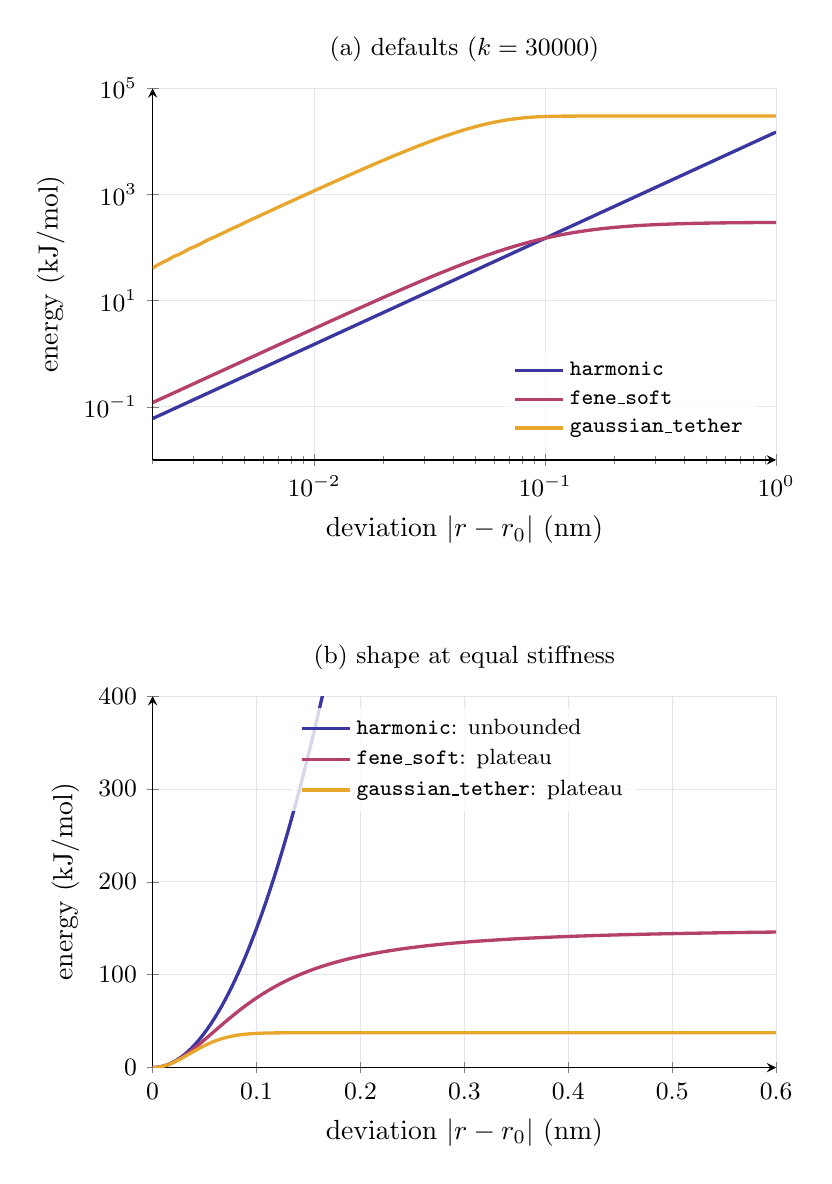
\begin{tikzpicture}
% (a) actual defaults, log-log
\begin{axis}[title={\small (a) defaults ($k=30000$)},xmode=log,ymode=log,
  xlabel={deviation $|r-r_0|$ (nm)},ylabel={energy (kJ/mol)},
  xmin=0.002,xmax=1,ymin=0.01,ymax=1e5,legend pos=south east,domain=0.002:1,samples=120]
\addplot[indigo] {15000*x^2};
\addlegendentry{\texttt{harmonic}}
\addplot[crimson] {30000*x^2/(1+100*x^2)};
\addlegendentry{\texttt{fene\_soft}}
\addplot[gold] {30000*(1-exp(-x^2/0.0025))};
\addlegendentry{\texttt{gaussian\_tether}}
\end{axis}
% (b) same initial stiffness, linear
\begin{axis}[at={(0,-3.0cm)},anchor=north west,title={\small (b) shape at equal stiffness},
  xlabel={deviation $|r-r_0|$ (nm)},ylabel={energy (kJ/mol)},
  xmin=0,xmax=0.6,ymin=0,ymax=400,domain=0:0.6,samples=200,clip=true,
  legend style={at={(0.5,0.97)},anchor=north}]
\addplot[indigo] {15000*x^2};
\addlegendentry{\texttt{harmonic}: unbounded}
\addplot[crimson] {15000*x^2/(1+100*x^2)};
\addlegendentry{\texttt{fene\_soft}: plateau}
\addplot[gold] {37.5*(1-exp(-x^2/0.0025))};
\addlegendentry{\texttt{gaussian\_tether}: plateau}
\end{axis}
\end{tikzpicture}
\end{document}
